\section{Architectural Design} % (fold)
\label{sec:architectural_design}

The biggest chunk of work -- measured in lines of code -- comes from the \idx{JavaScript} codebase.
All code from the \idx{Java} applet was ported to \idx{JavaScript}, adding more classes to the front-end code.
Most of the existing code was rewritten to seize specific features of \idx{MooTools}, and other classes needed to be added for the new elements.

At the same time, some code from the \ida{OSGi} bundle shifts to \ida{PHP} files, including all statics files needed to run the web application.
But the \ida{OSGi} bundle keeps being in charge of the \ida{TCP} socket, so it is as necessary as before.
Thankfully, the bundle does not need to be update and any build should work in both versions of the web application -- with and without the applet.

\subsection{JavaScript Codebase} % (fold)
\label{sub:javascript_codebase}

The basic design of the classes is pretty much the same as before, with all important elements of the interface having their respective classes to handle both the drawing and functionality behind that particular element.

All classes are implemented as \idx{MooTools} classes, to embrace its utilities and handy abstractions.
One of the things that are possible is to easily gain functionality from more than one class, by \emph{implementing} that \idx{MooTools} class (in reality it is more like extending).

Another pitfall was that the browser compatibility had to be very broad, and the codebase should remain the same for every browser.
The \idx{MooTools} library homogenized most of peculiarities, nevertheless some very specific hacks were needed for \idx{Internet Explorer}.
This became most handy in animations, but any \ida{DOM} homogenization is welcomed.

To avoid duplicity, it was decided that the same \idx{JavaScript} logic would handle the two interfaces.
Those designs are not just visually different, but they adopt very contrasting abstractions for interface elements and user actions.

The chosen solution was to dynamically load only the needed \idx{JavaScript} files depending on the platform.
It also results on two methods to create each one of the interfaces and diverted paths in the execution flow.
But that applies in few situations, and most of the code the same -- not similar but physically the same.

The \idx{Java} code for the applet was relatively straight to port to \idx{JavaScript}.
As figure~\ref{fig:class-pnai-java-port} shows, the model classes are very much alike, since they mostly contain data and methods to transform that data into a string that can be transmitted back to the server.

\begin{figure}[htbp]
  \centering
    \includegraphics[width=\textwidth]{diagrams/class-pnai-java-port.1}
  \caption{Class diagram for the new \idx{PNAI}: Model and BackendLink}
  \label{fig:class-pnai-java-port}
\end{figure}

The main difference is how the models are instantiated.
Before, the factory pattern was used to create objects from a string, but now that approach would have been more difficult to implement in \idx{JavaScript} and specially with \idx{MooTools} classes.
Now, the only way to create an object is directly \emph{instantiating} that object, even if no option is provided.
Later, the \idc{fromString()} functions can be used to parse any string and fill its options.

The other difference is related with the way the parameters of a class are given, something used in almost all classes.
This \idc{Options} interface -- provided by the \idx{MooTools} framework -- is a very powerful approach that allows the setting of any number of optional parameters in a class with only one line, without having to explicitly treat every value in the constructor.

About the \idc{BackendLink}, obviously the \idc{ScalenetApplet} class is gone, since that was the main class of the applet and now there is no applet.
Most of its functionality has been added to the \idc{BackendLink} class, so now it is in charge of all the communications with the backend.
This includes sending information to the \ida{TCP} socket and handling the data received in that socket, rerouting the actions as necessary.

One of the goals was to be able to change the \ida{APE} stuff with the applet by modifying as less code as possible.
A new, very simple class called \idc{AppletNotifier} now wraps all the code needed to use the \idc{BackendLink}.
By changing only a line of code there, the applet -- or any other new compatible system -- could be used again instead.
Basically it acts as a bridge between the logic of the application and the backend communications.

To maintain that possibility, some functions in the global object had to be kept because the applet directly calls them.
By design, no function should be declared in the global object, so they have been reduced to the minimum.
For obvious reasons, these functions have to keep the same parameters as before.

Apart from the backend link, the \idc{PendingAction} class keeps storing the data about the pending action, but now it is a little different.
In the application there is only one object of this class instantiated, \idc{ScaleNet.pending}, and that object is updated when necessary.
\idx{MooTools} offers \idc{Class.Occlude}, a class that makes this kind of singleton pattern very easy, by linking a \idx{MooTools} object to any \ida{DOM} element.

This brings us to one of the design decisions: to store all singleton objects in one place available from everywhere instead of using constructors to retrieve the cached objects.
This is to avoid some overhead and be faster in this very basic task.
As polluting the global object is seldom a good idea, there is a new object created in the global scope: \idc{ScaleNet}.

In the \idc{ScaleNet} object there are also defined all \idx{MooTools} classes, acting similarly to a \idx{Java} package in that the functionality is more compartmentalized.
Finally, that object contains some parameters to ease the development and customizability:

\begin{description}
  \item[ScaleNet.myIMPI] The user id, set by \ida{PHP} directly in the page.
  \item[ScaleNet.version] The version of the code (1.0), useful for future reference.
  \item[ScaleNet.desktop/ScaleNet.mobile] Booleans to indicate whether we are in the desktop version or the mobile one.
  Very useful to discriminate chunks of code depending on the context.
  \item[ScaleNet.debug] Boolean to activate debugging logs.
  \item[ScaleNet.zIndex] Needed for handling the position of the devices so that the newest ones appear on top of the oldest ones.
  \item[ScaleNet.host/ScaleNet.port] Host and port of the socket in the backend.
\end{description}

Figure~\ref{fig:class-pnai-containers} shows all code involving containers.
To deal with dimensions the new \idc{ContainerDimensions} class has been extracted from \idc{Container}, to homogenize and ease the work with positions and sizes across the application.
Also, it encapsulates all the logic needed to transform dimensions between pixels and percentages.

\begin{figure}[htbp]
  \centering
    \includegraphics[width=\textwidth]{diagrams/class-pnai-containers.1}
  \caption{Class diagram for the new \idx{PNAI}: Devices and Buddies}
  \label{fig:class-pnai-containers}
\end{figure}

The \idc{Container} class has received some improvements to implement the new functionality.
This includes the addition of functions to make the \ida{DOM} element both draggable and resizable.
These functions use some \idx{MooTools} classes for the hard work, but the dimensions are treated there to avoid \idx{Internet Explorer} glitches.

The device dimensions are defined in percentages, to be able to place the elements filling the page even if the user reopen the web application with a different window size.
\idx{Internet Explorer} does not like that, and the animations only works smoothly if the dimensions are specified in absolute units, i.e, pixels.
To avoid that bug, those functions automatically transform percentages to pixels at the beginning of the resizing/repositioning, and they change it back to percentages when the action is done.

The \idc{Container} class also demonstrates how the same code can handle two interfaces.
Since the created elements are very different, two functions are added to create the specific version -- \idc{createHTMLContainer()} for desktop and \idc{createMobileHTMLContainer()} for mobile.
Each of them uses \idx{MooTools} to dynamically create and add the elements to the \ida{DOM}.
When a container is created, the desktop/mobile flags can be checked so the correct method is called.

The last new method is called \texttt{pack()} and its goal is to resize the container to the available space.
This is needed for the desktop version because devices have to maintain the same aspect ratio, and because their sessions are drawn on top of the container -- in another element acting like a mask.
When the window size changes or when the element is resized, that mask needs to be repositioned and resized to the updated size.

Apart from that, the class implements the \idx{Events} class, another \idx{MooTools} addition that comes very handy to inject additional code in prefixed places in the class.
Basically, functions can be registered for some custom \emph{events}, in the code of the class the \idc{fireEvent} function is called when appropriate, so when that code is executed all registered functions are called.
For example, the \idc{enable} method fires the \texttt{enabled} event, so any other class can inject their code every time the \idc{enable} method is executed.

The \idc{DeviceList} class has been added to offer some functionality similar to the existing \idc{BuddyList} class.
The most important method is \idc{addDevices}, a function that populates the device list with the specified devices, ordering them so that they fill all available space (see Section~\ref{sec:positioning}).
Another function is provided to \emph{pack} every device at once, useful when resizing the window or the sidebar.
The rest is just the usual structure for handling a list.

\idc{BuddyList} and \idc{Buddy} are not very interesting, they just have been updated to \idx{MooTools} classes, but its functionality is mostly the same.
If something, the code has been simplified in favor of moving as much code as possible to the \idc{Container} class, to avoid duplicating code.

Figure~\ref{fig:class-pnai-sessions} comprises all classes around sessions and content items in general.
In the \idc{Session} class, the \idc{moveTo} method continues to be very important, since the visual representation of a session is not created until the session is moved to a container.
It is also in charge of moving sessions from a container to another, creating a nice animation using \idx{MooTools}.

\begin{figure}[htbp]
  \centering
    \includegraphics[width=\textwidth]{diagrams/class-pnai-sessions.1}
  \caption{Class diagram for the new \idx{PNAI}: Sessions and Content}
  \label{fig:class-pnai-sessions}
\end{figure}

A \idc{Session} is also draggable in the desktop version, so a similar method to the one in the \idc{Container} class is implemented.
Unlike containers, sessions should be prepared to be dropped, so the logic is a bit more complex.
The \idc{dropInto} method is called when the session is dropped into another valid container, and depending on the container it either requests the deletion of the session or it shows the popup menu.

The mobile version is much more straightforward, as the \idc{makeClickable} method just has to show the popup menu when the element is clicked.
\idc{SessionList} is another addition similar to other lists, and it just collects all the known sessions.

The \idc{Content} and \idc{ContentList} classes are completely new, as the functionality was simply not there.
\idc{Content} stores all information about a particular piece of content, and also includes the needed code to handle purchases of that content.

In the desktop there are two approaches: to directly buy the piece by clicking the \emph{Buy} button, or by dragging the icon to a specific container.
For the second approach the system is very similar to dragging sessions, with a method to add the dragging functionality and another to handle a successful action.
In both situations, a confirmation popup will appear -- the \texttt{options.link} sets the address to open.
One important difference is that, when the user drags the icon to the buddies tab, that tab gets revealed.

In the mobile version the \idc{createMobileHTMLContainer} method handles the whole \emph{tap twice to buy the content} experience, and the posterior selection of a target.
Because of that, this method is somewhat complex, but since it does not need any additional confirmation, it can directly tell the backend that the user wants to buy that content -- for that the address contacted in the \ida{AJAX} call is the one stored in the \texttt{options.ajaxlink} property.

There is one last interesting detail about this class: when a new piece of content is created, it traverses the current session list and updates the session icon with the thumb icon for that content.
This means that, when the content is loaded, the current sessions get their characteristic icons, even if that information was not provided by the \ida{OSGi} bundle through the socket.
However, if there is a problem and the content is not loaded, the current sessions will not have custom icons.

The \idc{ContentList} class is in charge of not only collecting and categorizing the pieces of content, but also of preparing the interface for that content list.
The \idc{loadContent} method is the most important one, since it dynamically retrieves that list from the server after the page is loaded.
The information is obtained with a \ida{JSONP} request to a \idx{PHP} page.

Figure~\ref{fig:class-pnai-interface} gathers the rest of the classes in the \idx{JavaScript} codebase, mostly related with interface elements and their behavior.
The \idc{PopupMenu} class is in charge of showing the popup menu to the user with the available options -- transfer, duplicate and stop sessions --, and react to the user selection.
In that occasions, the \idx{AppletNotifier} is created on demand.
In the mobile version, this class also is in charge of the select destination mode.

\begin{figure}[htbp]
  \centering
    \includegraphics[width=\textwidth]{diagrams/class-pnai-interface.1}
  \caption{Class diagram for the new \idx{PNAI}: Interface elements}
  \label{fig:class-pnai-interface}
\end{figure}

The \idc{InfoPanel} class is responsible of showing the informational panel to provide feedback to the user.
There are two different types of messages: normal messages and errors; each of them have different icons to alert the user depending on the result.
The interesting bit about this class is that it allows the chaining of messages, so that every message is shown to the user at least for a couple of seconds even if they are triggered at the same time.

In the desktop version a third party \idx{MooTools} class is used, called \idc{Growl}\footnote{\url{http://icebeat.bitacoras.com/mootools/growl/}} because it emulates the looks of a notification system for Mac.
Though some little fixes had to be added to make it compatible with the latest version of \idx{MooTools}, it automatically handles the chaining of messages.

However, in the mobile version another approach was needed, because the previous class was designed for desktop browsers but not for mobile browsers.
It was more efficient to do it by hand, therefore a very basic notification system was implemented allowing also the chaining of messages with a simple but elegant look.

The \idc{Drawer} class is specific to the desktop interface, and it manages all aspects regarding the sidebar, such as tabbed navigation.
It also deals with its resizing and visibility, something that needed a lot of attention to fix quirky bugs in \idx{Internet Explorer}.

Its mobile counterpart is the \idc{BarTab} class, that administers the navigation system based on the bottom tabs and nearly everything related in the mobile interface, like orientation changes.
To successfully implement the tab bar, it uses \idx{iScroll}, another \idx{JavaScript} component designed for \idx{Webkit} mobile browsers (see Section~\ref{sec:mobile}).
% subsection javascript_codebase (end)

\subsection{PHP Codebase} % (fold)
\label{sub:php_codebase}

In the server all modified code is implemented in \ida{PHP} scripts, sharing the same tree as the \idx{IPTVplus} interface.
Figure~\ref{fig:phpdir} shows all the new files in bold, in contrast to Section~\ref{sub:iptvplus}
The main page remains mostly the same, just updating some styles to modernize and fix some bugs without changing the overall style.

\begin{figure}[htbp]
  \dirtree{%
    .1 scalenet/.
      .2 index.php.
      .2 sub/.
        .3 includes/.
          .4 \textbf{c2d-ajax.php}.
          .4 c2d.php.
          .4 inhalt.php.
          .4 popup.php.
        .3 IPTVplus.php.
        .3 \textbf{IPTVplusJSON.php}.
        .3 personal/.
          .4 sessions.php.
        .3 personal.php.
        .3 \textbf{pnai/}.
          .4 \textbf{cache.manifest}.
          .4 \textbf{css/}.
          .4 \textbf{desktop.php}.
          .4 \textbf{images/}.
          .4 \textbf{index.php}.
          .4 \textbf{js/}.
            .5 \textbf{ape-jsf/}.
            .5 \textbf{appletglue.js}.
            .5 \textbf{backendlink.js}.
            .5 \textbf{bartab.js}.
            .5 \textbf{buddies.js}.
            .5 \textbf{containers.js}.
            .5 \textbf{content.js}.
            .5 \textbf{iscroll/}.
            .5 \textbf{main-mobile.js}.
            .5 \textbf{main.js}.
            .5 \textbf{model.js}.
            .5 \textbf{mootools-1.2.4-core-yc.js}.
            .5 \textbf{mootools-1.2.4.4-more.js}.
            .5 \textbf{notifications.js}.
            .5 \textbf{sessions.js}.
            .5 \textbf{sidebar.js}.
            .5 \textbf{util.js}.
          .4 \textbf{mobile-auth.inc.php}.
          .4 \textbf{mobile.php}.
  }
  \caption{New PHP directory}
  \label{fig:phpdir}
\end{figure}

In the desktop, the user starts visiting the \texttt{index.php} (see Figure~\ref{fig:scalenet-frontpage}), where he can choose between the old \idx{IPTVplus} application, the \ida{PNAI} (at the right) and another different application, the MeshBed.
Once the user clicks on the \emph{myNetwork} link, the \texttt{personal.php} page presents a login form (see Figure~\ref{fig:scalenet-login}).

\begin{figure}[htbp]
  \centering
    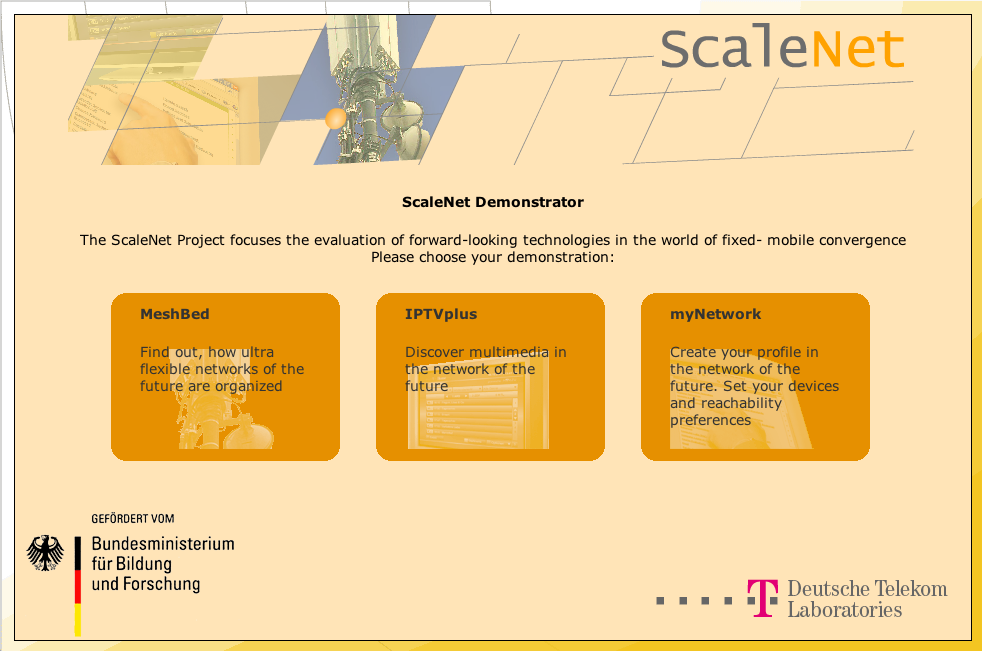
\includegraphics[width=\textwidth]{scalenet-frontpage}
  \caption{ScaleNet front page}
  \label{fig:scalenet-frontpage}
\end{figure}

\begin{figure}[htbp]
  \centering
    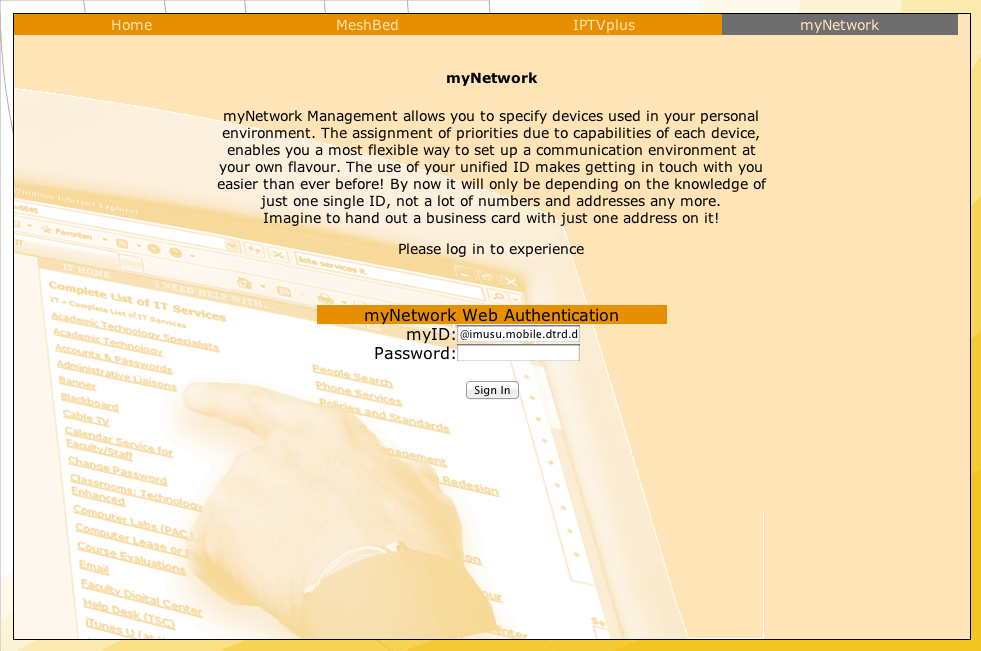
\includegraphics[width=\textwidth]{scalenet-login}
  \caption{ScaleNet login page}
  \label{fig:scalenet-login}
\end{figure}

If the user logs in successfully, that page will change to include the \idc{session.php} page.
In that page a frame is defined: previously it linked to the server built by the \idx{OSGi} bundle, but now it just links to the \texttt{desktop.php} page in the \texttt{pnai} directory.
The whole picture looks like Figure~\ref{fig:pnai-buddies}.

However, if the user try to visit the front page from an \idx{iOS} or \idx{Android} device, he will be redirected to the \idx{mobile.php} page in the \texttt{pnai} directory.
If the user is not logged in, the \texttt{mobile-auth.inc.php} displays the login form (see Figure~\ref{fig:pnai-mobile-login}), but if he is already logged in, his devices are directly shown (see Figure~\ref{fig:pnai-mobile-devices}).

That way, all code related to the new \ida{PNAI} is all isolated in the \idx{pnai} directory.
Both \texttt{desktop.php} and \texttt{mobile.php} are the respective main pages for the two interfaces, and they define only some basic elements needed in the page structure.
In the \texttt{css} directory all the styles are stored in two different files -- one for each file.
Also, that directory contains the web fonts used for some effects.
Finishing with the assets, the \texttt{images} directory stores all the needed art files for the interface.

Finally, the \texttt{js} directory is the home for all \idx{JavaScript} code.
Each file includes one or more \idx{MooTools} classes organized by topic.
Most of them are self explanatory, except \texttt{utils.js} that defines the \idc{InfoPanel} and \idc{PopupMenu} classes.

The desktop version includes all files except \texttt{bartab.js} -- that contains only that class --, \texttt{iscroll} -- the third party library --, and \texttt{main-mobile.js} -- the main function that prepares all.
The mobile version includes all files except \texttt{sidebar.js} -- the \texttt{Drawer} class --, \texttt{notifications.js} -- the \idx{Growl} library --, and \texttt{main.js} -- the desktop version of that main function.

The last file to explain, and probably the less important, is \idx{cache.manifest}.
This file is used to help the mobile browser caching the application static assets -- \idx{JavaScript}, \ida{CSS} and images.
Its content is basically a plain list of all static resources.

Going up to the \texttt{sub} directory, there are two new \ida{PHP} scripts.
Both are designed as the \ida{AJAX} versions of other two scripts, so their output is formatted in \ida{JSON}/\ida{JSONP} instead of \ida{HTML}.
\texttt{IPTVplusJSON.php} returns the list of contents available to buy and \texttt{c2d-ajax.php} receives purchase requests so the content can start streaming.

Both connects to the \ida{IMS} server through a socket, then they send a command, the \ida{IMS} responds and then they format the output accordingly.
\texttt{IPTVplusJSON.php} sends the \texttt{list} command, it receives the content list in a string where every new line is a new content, and it formats it like in Listing~\ref{iptvplusjson}.
It is no surprise that it contains exactly the same information as in the \idc{Content} \idx{MooTools} class.

\begin{lstlisting}[language=JavaScript,label=iptvplusjson,caption=JSON content list example]
myCallback({
  "error": false,
  "content": [
    {
      "id": "MYID",
      "img": "/scalenet/sub/iptvplus/images/...jpg",
      "title": "Content title",
      "type": "tv",
      "priority": "everybody",
      "price": "3",
      "desc": "Content description",
      "quality": "100\/300\/...2000\/4000",
      "link": "popup.php?price=3&link=c2d.php?%3Ftype%3Dtv%26...",
      "ajaxlink": "c2d-ajax.php?type=tv&quality=...&content=MYID&impu="
    },
    {...}
  ]
});
\end{lstlisting}

The response, a \idx{JavaScript} object, is wrapped into a function call which name is defined by passing a parameter to the script.
One of the properties of that object is \texttt{error}, that contains a message for the user if the content list could not be retrieved.
The main property is \texttt{content}, an array made by objects with the required data for each piece of content.

As explained before, the \texttt{link} is used by the desktop version and the \texttt{ajaxlink} by the mobile version.
Each of one is already prepared to be called with all parameters except the destination \texttt{impu}.
Consequently, the \texttt{c2d-ajax.php} script receives that request with those parameters, then it opens the socket and sends a \texttt{refer} command.
The response to the browser is the \texttt{error} message in case of a problem or simply an object with the content \texttt{\{result:~'OK'\}} in case of success.
% subsection php_codebase (end)
% section architectural_design (end)